% !TEX root =  ../supplementary.tex
\section{Simulation Study}
\subsection{Simulation Results for Dynamic Risk of GR Based Approach With a Fixed $\kappa = 0.95$}
In the main manuscript, for the personalized schedules based on dynamic risk of GR we chose $\kappa$ on the basis of $\mbox{F}_1$ score. However while conducting the simulation study, we also tried a fixed $\kappa$ of 0.95, which means that the next biopsy is scheduled at a time point where the dynamic risk of GR is 5\%. The results for this approach are presented in \ref{table : sim_study_pooled_estimates_extended}. In the table, the abbreviation Dyn. risk GR ($\mbox{F}_1$ score) corresponds to personalized schedules based on dynamic risk of GR based approach, with $\kappa$ chosen on the basis of $\mbox{F}_1$ score. The abbreviation Hybrid ($\mbox{F}_1$ score) corresponds to the hybrid approach between median time of GR and dynamic risk of GR ($\kappa$ chosen on the basis of $\mbox{F}_1$ score).

\begin{table}[!htb]
\caption{Estimated mean and standard deviation (SD), of the number of biopsies $N^S_j$ conducted until Gleason reclassification (GR) is detected, and of the offset $O^S_j$ (difference in time at which GR is detected and the true time of GR, in months), for the simulated (500 datasets) test patients, across different schedules and subgroups. Patients in subgroup $G_1$ have the fastest prostate cancer progression rate, whereas patients in subgroup $G_3$ have the slowest progression rate. Types of personalized schedules (full names in brackets): Exp. GR Time (expected time of GR), Med. GR Time (median time of GR), Dyn. risk GR (schedules based on dynamic risk of GR), Hybrid (a hybrid approach between median time of GR and dynamic risk of GR). Annual corresponds to a schedule of yearly biopsies and PRIAS corresponds to biopsies as per PRIAS protocol.}
\label{table : sim_study_pooled_estimates_extended}
\begin{tabular}{lrrrr}
\Hline
\multicolumn{5}{c}{a) All hypothetical subgroups}\\
\hline
Schedule          & $E(N^S_j)$ & $E(O^S_j)$ & ${\mbox{SD}(N^S_j)}$ & ${\mbox{SD}(O^S_j)}$ \\
\hline
Annual         & 5.24            & 6.01                & 2.53          & 3.46              \\
PRIAS          & 4.90            & 7.71                & 2.36          & 6.31\\
Dyn. risk GR ($\mbox{F}_1$ score)       & 4.69            & 6.66                & 2.19           & 4.38              \\
Hybrid ($\mbox{F}_1$ score)      & 3.75            & 9.70                & 1.71          & 7.25              \\
Dyn. risk GR ($\kappa=0.95$) & 5.15 & 6.02 & 2.51 & 3.47\\
Med. GR time & 2.06            & 13.88               & 1.41          & 11.80              \\
Exp. GR time & 1.92            & 15.08               & 1.19          & 12.11             \\
\hline
\multicolumn{5}{c}{b) Hypothetical subgroup $G_1$}\\
\hline
Schedule        & $E(N^S_j)$ & $E(O^S_j)$ & ${\mbox{SD}(N^S_j)}$ & ${\mbox{SD}(O^S_j)}$ \\
\hline
Annual         & 4.32            & 6.02                & 3.13          & 3.44              \\
PRIAS          & 4.07            & 7.44                & 2.88          & 6.11    \\
Dyn. risk GR ($\mbox{F}_1$ score)       & 3.85            & 6.75                & 2.69          & 4.44              \\
Hybrid ($\mbox{F}_1$ score)       & 3.25            & 10.25               & 2.16          & 8.07              \\
Dyn. risk GR ($\kappa=0.95$) & 4.23 & 6.05 & 3.10 & 3.46\\
Med. GR time & 1.84            & 20.66               & 1.76          & 14.62             \\
Exp. GR time & 1.72            & 21.65               & 1.47          & 14.75             \\
\hline      
\multicolumn{5}{c}{c) Hypothetical subgroup $G_2$}\\
\hline
Schedule        & $E(N^S_j)$ & $E(O^S_j)$ & ${\mbox{SD}(N^S_j)}$ & ${\mbox{SD}(O^S_j)}$ \\
\hline
Annual         & 5.18            & 5.98                & 2.13          & 3.47              \\
PRIAS          & 4.85            & 7.70                & 2.00          & 6.29        \\
Dyn. risk GR ($\mbox{F}_1$ score)       & 4.63            & 6.66                & 1.82          & 4.37              \\
Hybrid ($\mbox{F}_1$ score)       & 3.68            & 10.32                & 1.37          & 7.45              \\
Dyn. risk GR ($\kappa=0.95$) & 5.09 & 5.99 & 2.11 & 3.47\\
Med. GR time & 1.89             & 12.33               & 1.16          & 9.44              \\
Exp. GR time & 1.77            & 13.54               & 0.98          & 9.83              \\
\hline      
\multicolumn{5}{c}{d) Hypothetical subgroup $G_3$}\\
\hline
Schedule        & $E(N^S_j)$ & $E(O^S_j)$ & ${\mbox{SD}(N^S_j)}$ & ${\mbox{SD}(O^S_j)}$ \\
\hline
Annual         & 6.20             & 6.02                & 1.76          & 3.46              \\
PRIAS          & 5.76             & 7.98                & 1.71         & 6.51        \\
Dyn. risk GR ($\mbox{F}_1$ score)       & 5.58            & 6.58                & 1.56          & 4.33              \\
Hybrid ($\mbox{F}_1$ score)       & 4.32            & 8.55                & 1.26          & 5.91              \\
Dyn. risk GR ($\kappa=0.95$) & 6.11 & 6.01 & 1.76 & 3.46\\
Med. GR time & 2.45            & 8.70                & 1.15          & 6.32              \\
Exp. GR time & 2.27            & 10.09               & 0.99          & 7.47              \\
\hline     
\end{tabular}
\end{table}

\clearpage

\subsection{Variation in Estimated Mean and Standard Deviation, of Number of Biopsies and Offset Across the 500 Simulations}
In this section we present figures related to the simulation study results discussed in Section \ref{sec: simulation_study} of main manuscript. The figures we present next are population specific, i.e. subgroup level differentiation is not done.

\begin{itemize}
  \item Variation in estimated mean across the 500 simulations, for number of biopsies and offset (difference in time at which Gleason reclassification or GR is detected and the true time of GR, in months) for different methods is shown in Web Figure \ref{fig : nbMeanBoxPlot_all} and Web Figure \ref{fig : offsetMeanBoxPlot_all}.
  \item Variation in estimated standard deviation across the 500 simulations, for number of biopsies and offset (difference in time at which Gleason reclassification or GR is detected and the true time of GR, in months) for different methods is shown in Web Figure \ref{fig : nbSDBoxPlot_all} and Web Figure \ref{fig : offsetSDBoxPlot_all}.
\end{itemize}

\begin{figure}[!htb]
\centerline{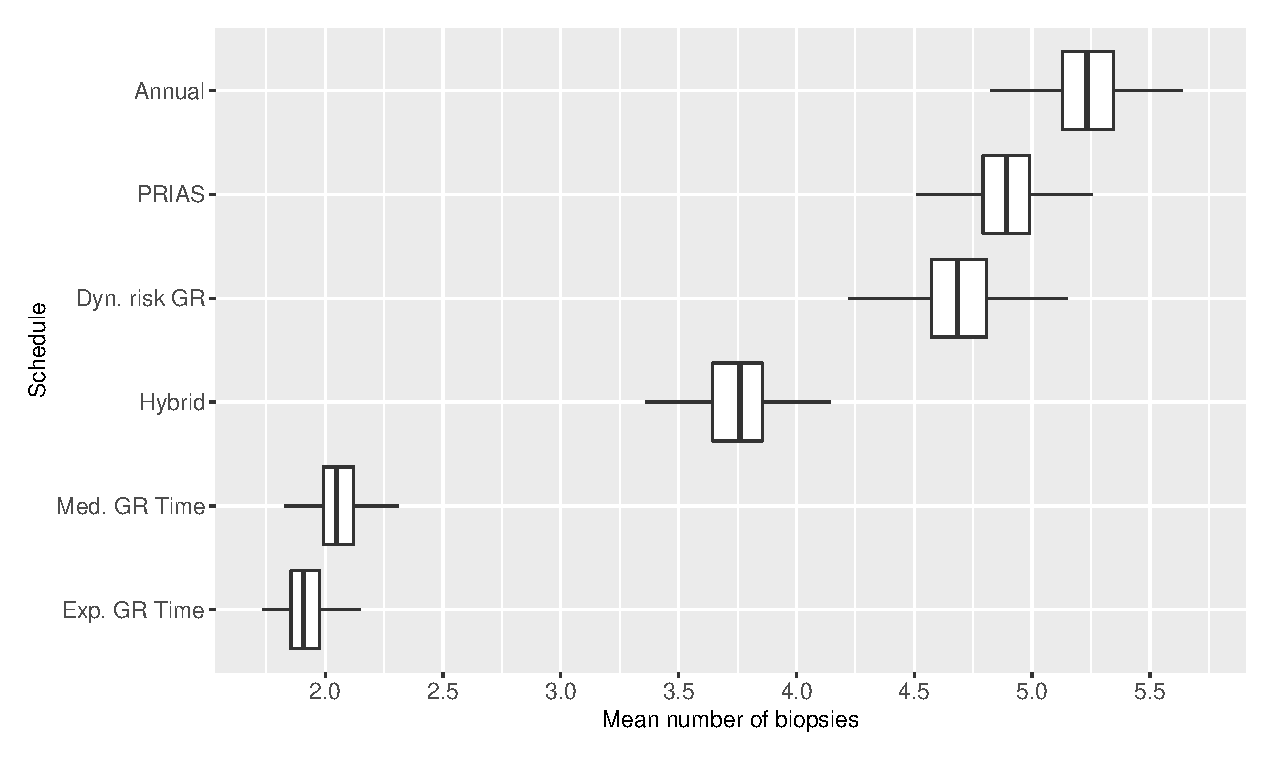
\includegraphics[width=\columnwidth]{images/sim_study/nbMeanBoxPlot_all.eps}}
\caption{Boxplot showing variation in estimated mean number of biopsies conducted by various schedules until Gleason reclassification is detected, obtained from the simulation study with 500 simulated datasets.}
\label{fig : nbMeanBoxPlot_all}
\end{figure}

\begin{figure}[!htb]
\centerline{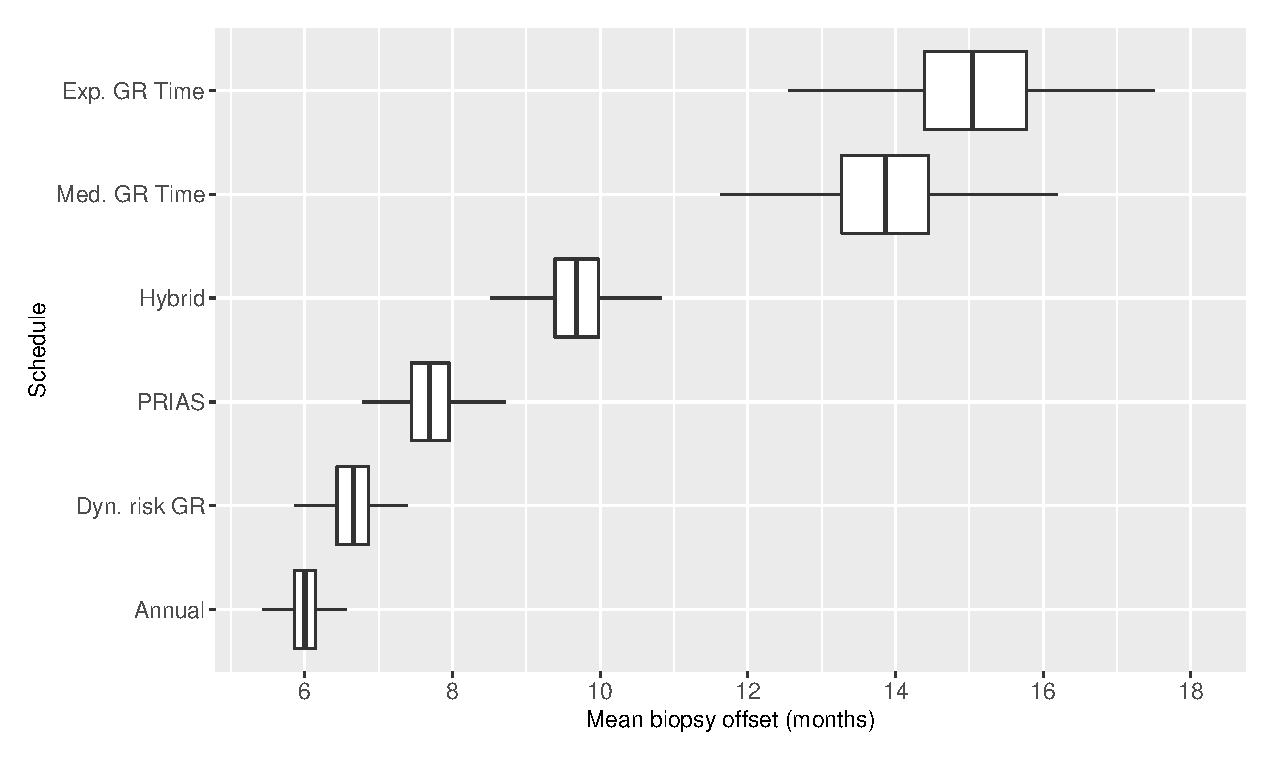
\includegraphics[width=\columnwidth]{images/sim_study/offsetMeanBoxPlot_all.eps}}
\caption{Boxplot showing variation in estimated mean of biopsy offset (difference in time at which Gleason reclassification or GR is detected and the true time of GR, in months) for various schedules, obtained from the simulation study with 500 simulated datasets.}
\label{fig : offsetMeanBoxPlot_all}
\end{figure}

\begin{figure}[!htb]
\centerline{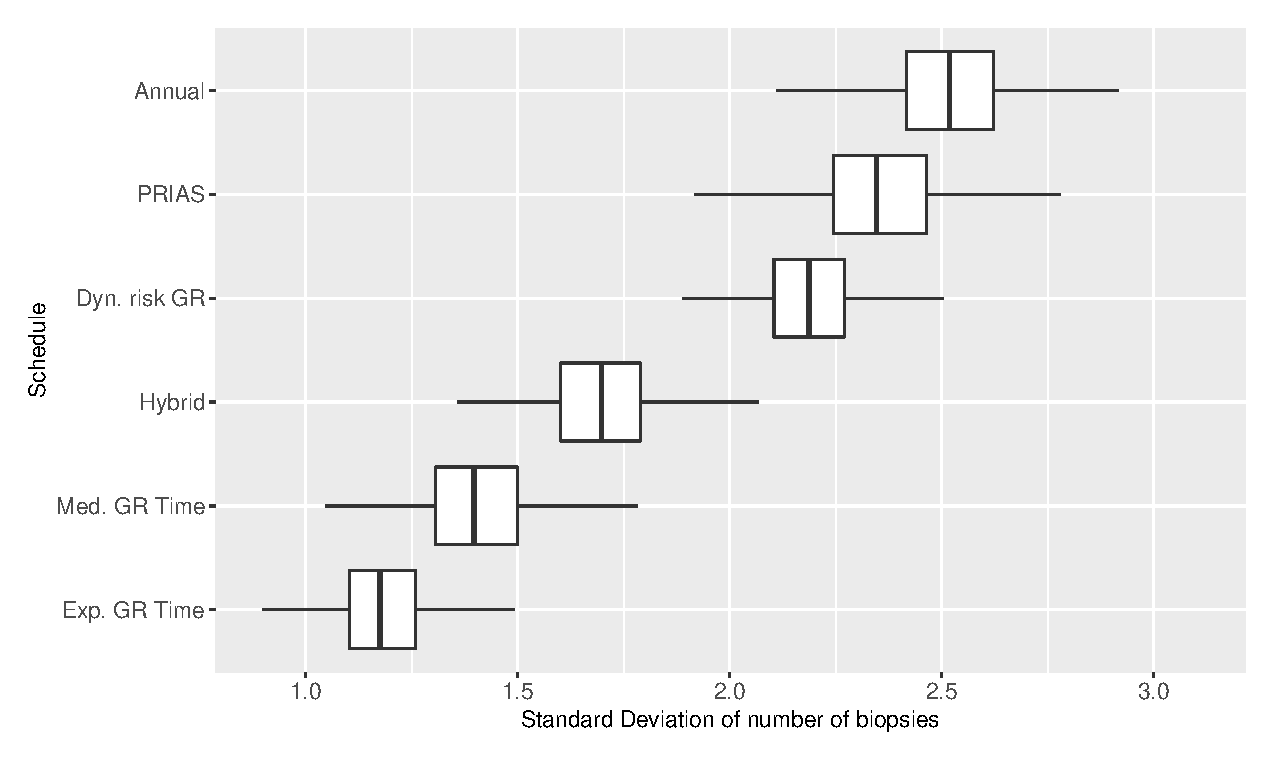
\includegraphics[width=\columnwidth]{images/sim_study/nbSDBoxPlot_all.eps}}
\caption{Boxplot showing variation in estimated standard deviation of number of biopsies conducted by various schedules until Gleason reclassification is detected, obtained from the simulation study with 500 simulated datasets.}
\label{fig : nbSDBoxPlot_all}
\end{figure}

\begin{figure}[!htb]
\centerline{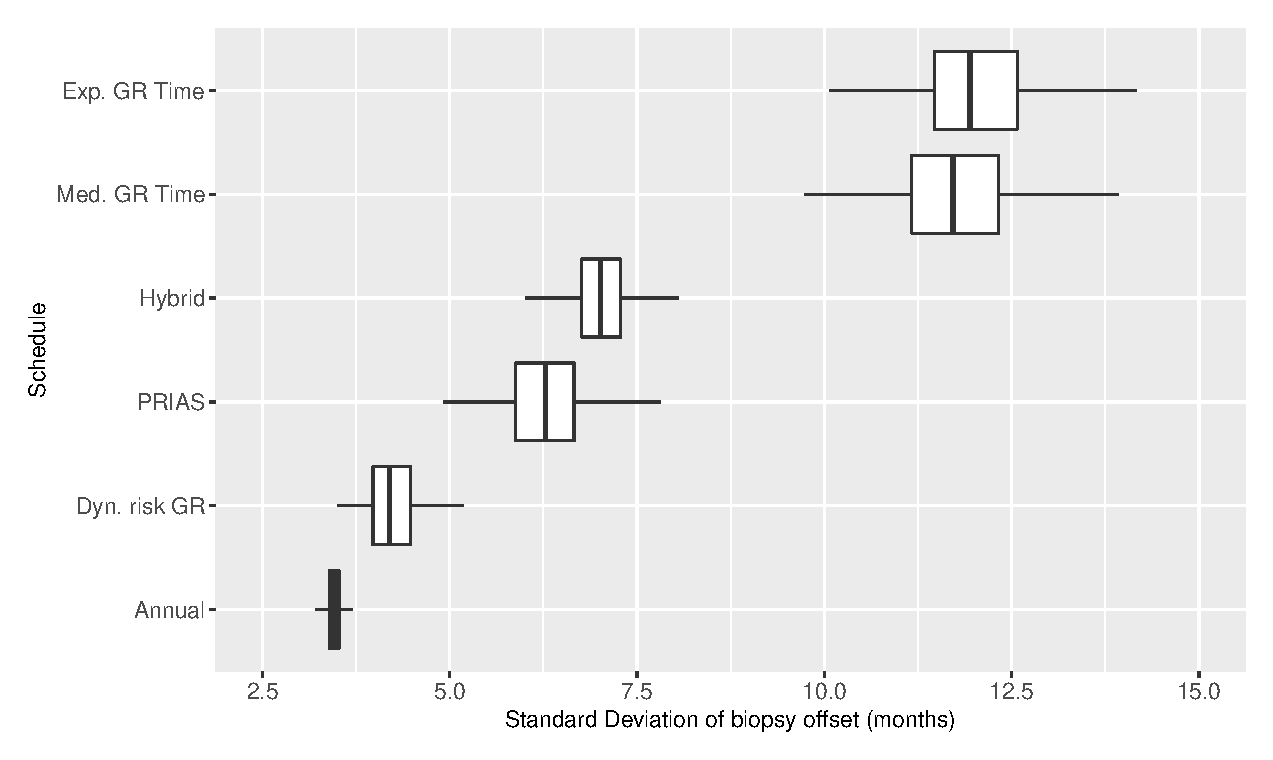
\includegraphics[width=\columnwidth]{images/sim_study/offsetSDBoxPlot_all.eps}}
\caption{Boxplot showing variation in estimated standard deviation of biopsy offset (difference in time at which Gleason reclassification or GR is detected and the true time of GR, in months) for various schedules, obtained from the simulation study with 500 simulated datasets.}
\label{fig : offsetSDBoxPlot_all}
\end{figure}



